A \Figref{grafico-resultados} compara os resultados de simulação e experimentais
sobre a mesma referência. Adotando o \gls{rmse} (\Eqref{rmse}) sobre o erro de
seguimento da temperatura relativa do sensor~2, o sistema simulado apresentou
$\mathrm{RMSE} = 1{,}3567\,^\circ\mathrm{C}$ e o ensaio experimental
$\mathrm{RMSE} = 2{,}2956\,^\circ\mathrm{C}$. Em ambos os casos a estratégia
\gls{pd} com \gls{ff} acompanhou a referência no transitório e em regime
permanente, recuperando-se após a perturbação aos 10 minutos.

\begin{figure}[H]
\centering
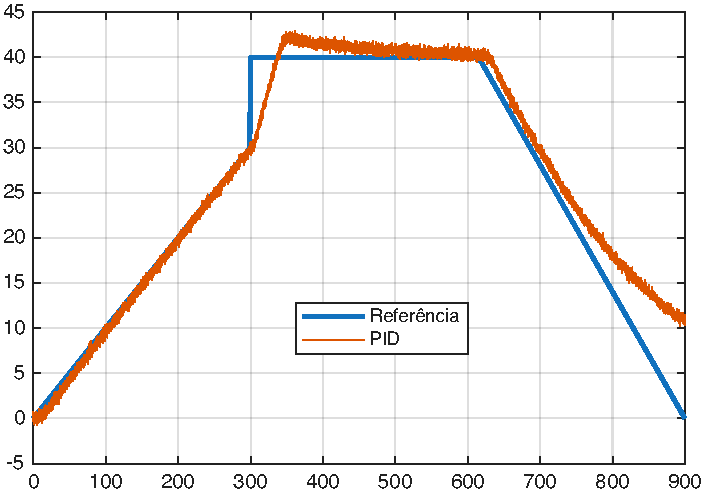
\includegraphics[width=0.9\linewidth]{images/Resultados.pdf}
\caption{Comparação entre os resultados simulado e experimental quanto ao
seguimento da referência de temperatura relativa do sensor~2.}
\figlabel{grafico-resultados}
\end{figure}